\chapter{Experimental Results}
High-speed flight in the wild is very challenging because of their complex structure (e.g. thick vegetation, thin branches, or collapsed walls) and multiple options available to avoid obstacles. In addition, a high-level understanding of the environment is necessary, which is worsened by challenging illumination conditions and low texture surfaces (e.g. because of snow). 

The experiments in simulation show that the proposed approach reduces the failure rate up to 10 times with respect to state-of-the-art methods. The results are confirmed by testing in a variety of real-world environments using a custom-built physical quadrotor; deploying the policy trained in simulation without any further adaptations. 

\section{Environmental Setup}
In all experiments conducted, the drone was provided with a reference trajectory to encode the intended flight path. The trajectories are not collision-free and would lead to a crash into obstacles if blindly executed. This reference can be provided by a user or a higher-level planning algorithm. The drone is tasked to follow that flight path and make adjustments as necessary to avoid obstacles. 

The performance is measured according to success rate, i.e. the percentage of successful runs over the total number of runs, where it is considered as a successful run if the drone reaches the goal location within a radius of 5 m without crashing. 

\subsection{Natural environment}
Experiments are performed in diverse natural environments as shown in figure \ref{fig:natural envt}. The experiment were performed in two different reference trajectories: a 40 m-long straight line and a circle with a 6 m radius. The quadrotor was flown in a straight line at different average speeds in the range of 3 to 10 $m/s$. A total of 31 experiments were conducted in natural environments.

\begin{figure}[!h]
	\centering
	\begin{subfigure}[b]{0.29\textwidth}
		\centering
		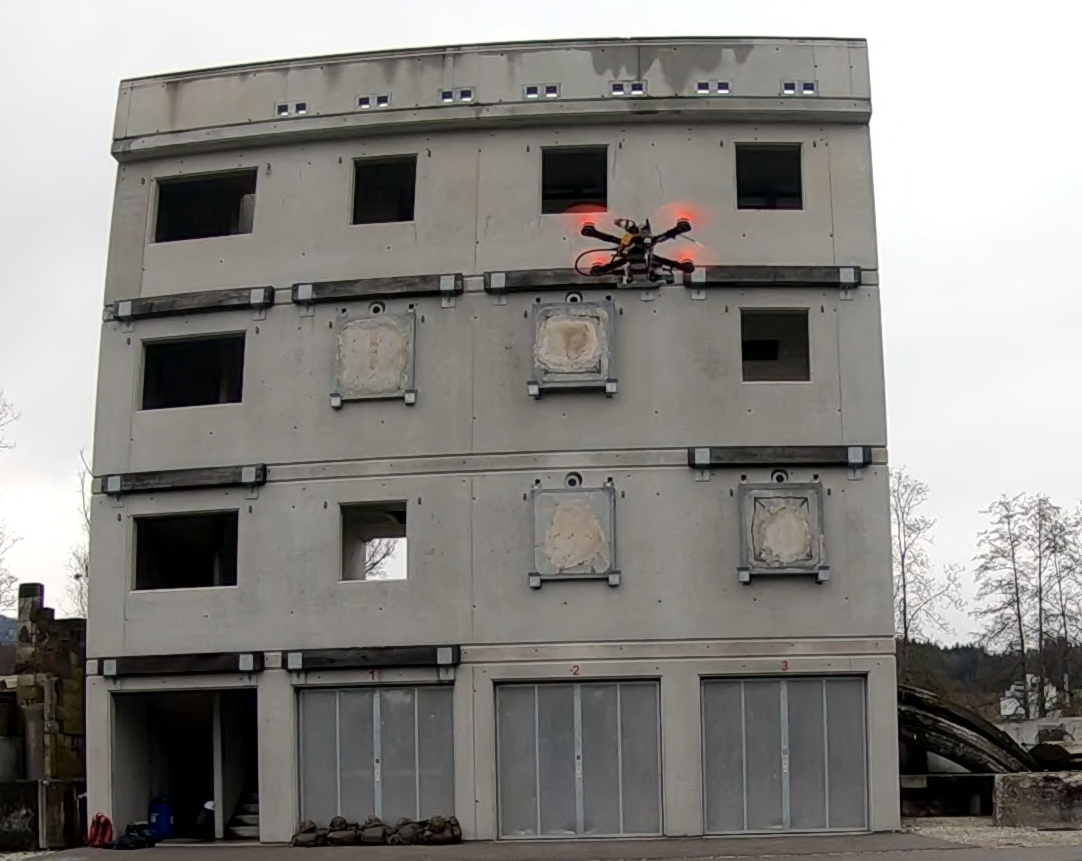
\includegraphics[keepaspectratio=true, width=\textwidth]{Navigation Environment/building.png}
		\caption{Building}
	\end{subfigure}
	\hfill
	\begin{subfigure}[b]{0.29\textwidth}
		\centering
		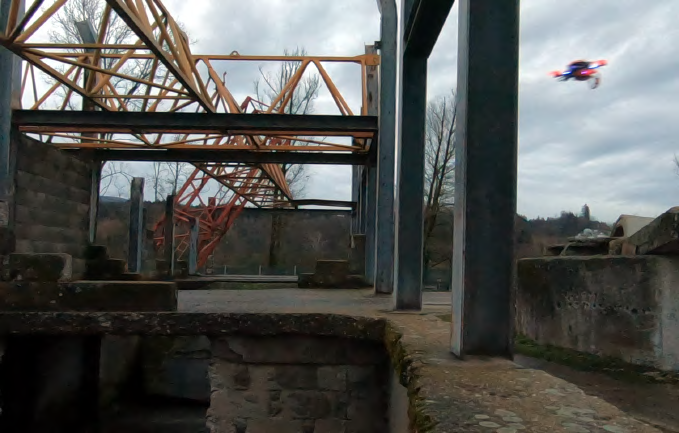
\includegraphics[keepaspectratio=true, width=\textwidth]{Navigation Environment/collapsed building.png}
		\caption{Collapsed Building}
	\end{subfigure}
	\hfill	
	\begin{subfigure}[b]{0.29\textwidth}
		\centering
		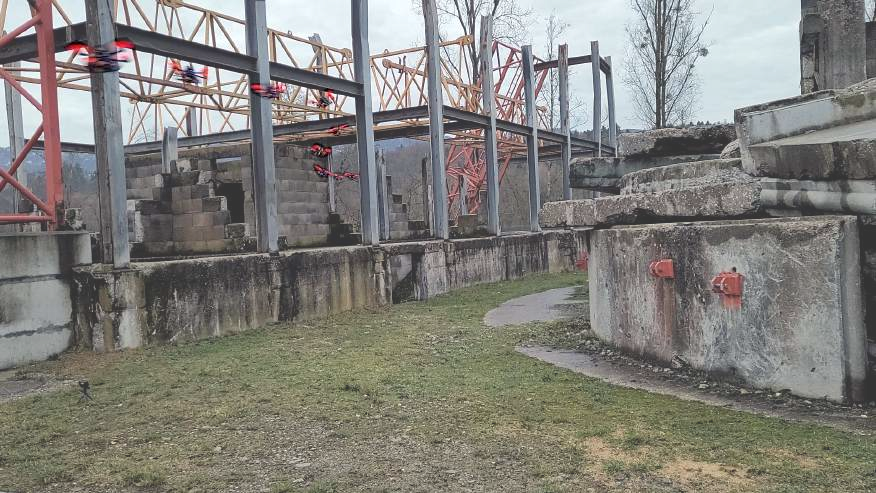
\includegraphics[keepaspectratio=true, width=\textwidth]{Navigation Environment/construction site.png}
		\caption{Construction site}
	\end{subfigure}
	\hfill
	\begin{subfigure}[b]{0.29\textwidth}
		\centering
		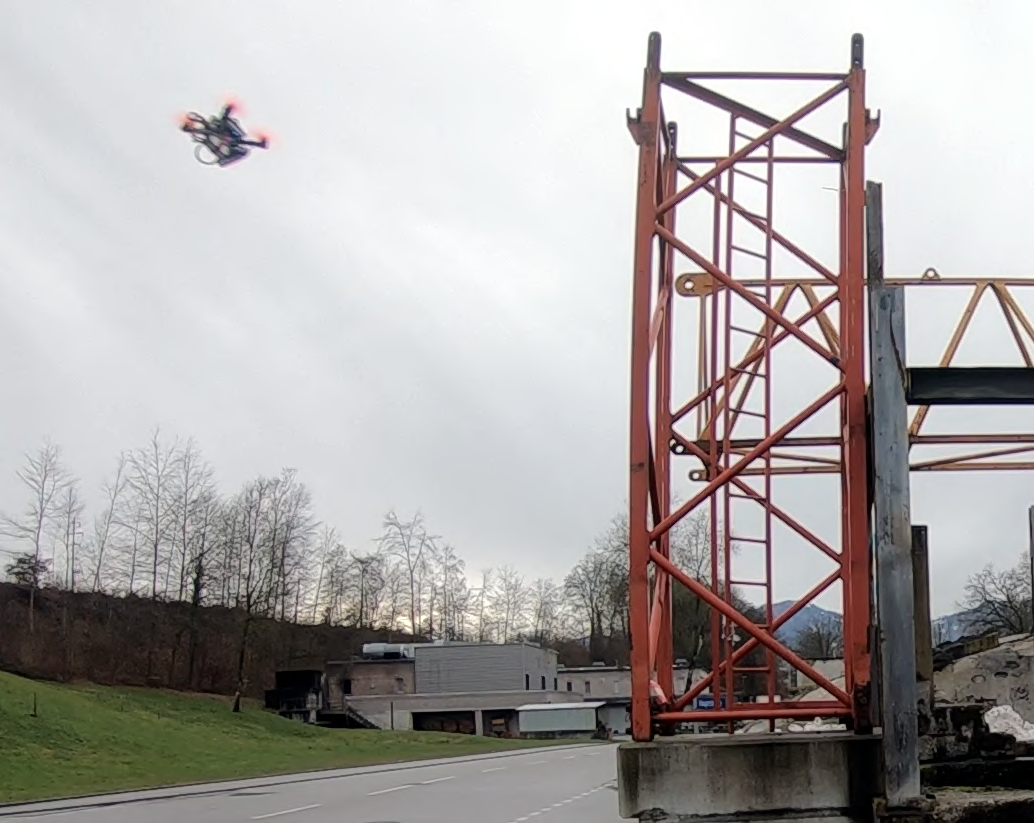
\includegraphics[keepaspectratio=true, width=\textwidth]{Navigation Environment/crane.png}
		\caption{Crane}
	\end{subfigure}
	\hfill
	\begin{subfigure}[b]{0.29\textwidth}
		\centering
		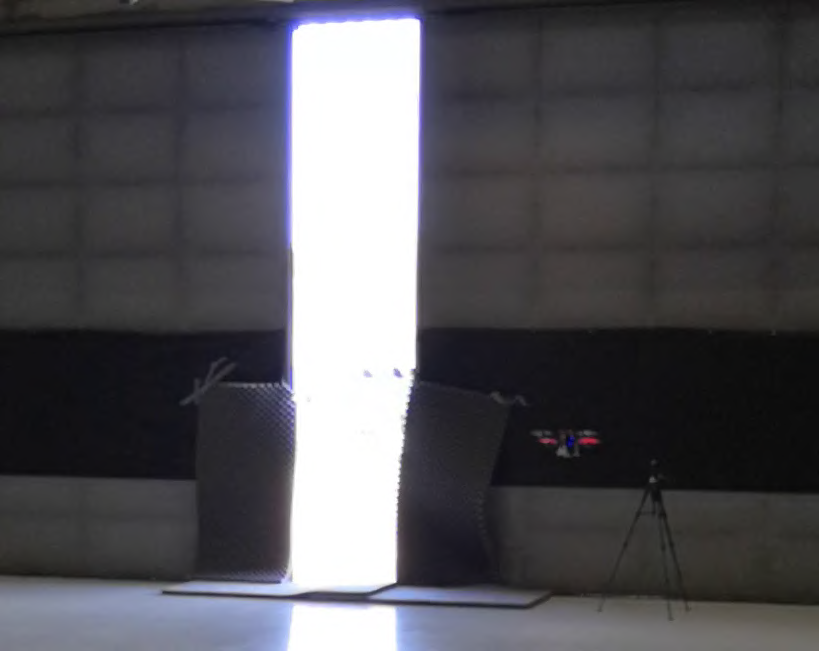
\includegraphics[keepaspectratio=true, width=\textwidth]{Navigation Environment/narrow gap(2).png}
		\caption{Narrow gap}
	\end{subfigure}
	\hfill
	\begin{subfigure}[b]{0.29\textwidth}
		\centering
		\includegraphics[keepaspectratio=true, width=\textwidth]{Navigation Environment/Ruins.png}
		\caption{Ruins}
	\end{subfigure}
	
	\caption{Human-made environment test fields}
	\label{fig:human envt}
\end{figure}


\subsection{Human-made environments}
In these environments, the drone faces a different set of challenges. It has to avoid obstacles with a variety of sizes and shapes as shown in figure \ref{fig:human envt}. The irregular and/or large structure of the encountered obstacles, the limited number of flyable openings, and the requirement to initiate the avoidance maneuver well in advance, offer a complementary set of challenges.

\begin{figure}[!h]
	\centering
	\begin{subfigure}[b]{0.29\textwidth}
		\centering
		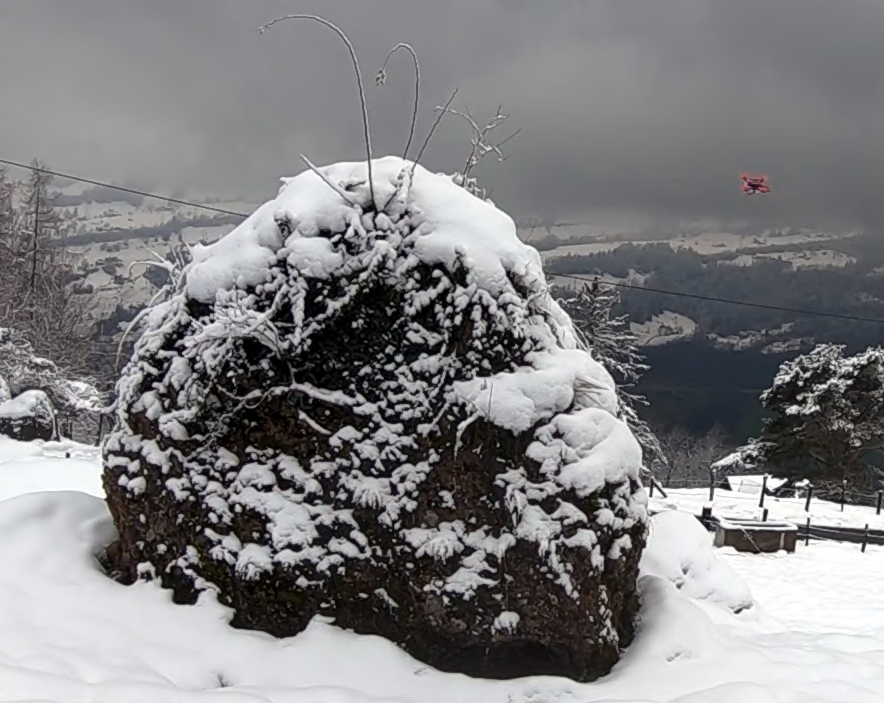
\includegraphics[keepaspectratio=true, width=\textwidth]{Navigation Environment/Boulder.png}
		\caption{Snowy Environment}
	\end{subfigure}
	\hfill
	\begin{subfigure}[b]{0.29\textwidth}
		\centering
		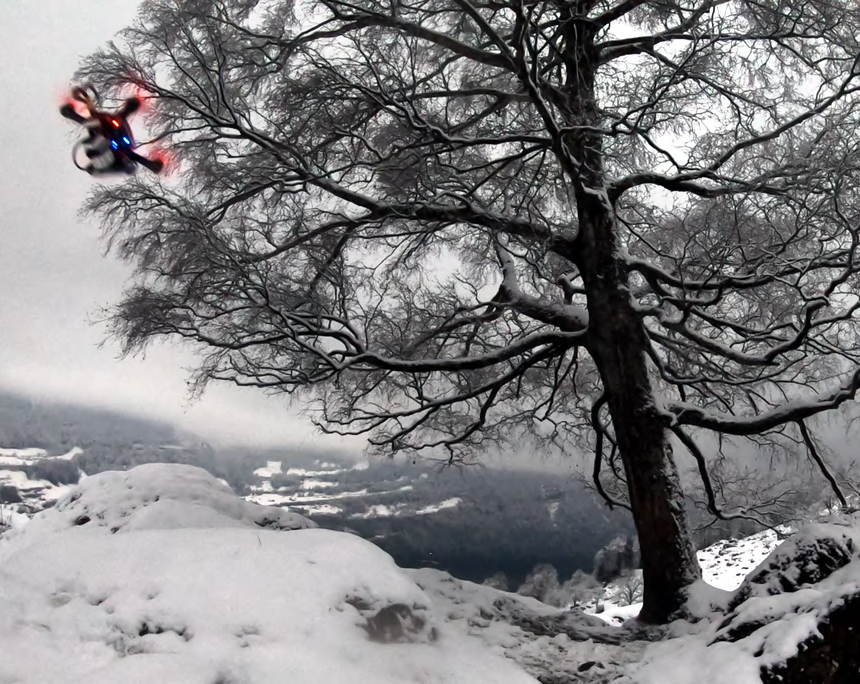
\includegraphics[keepaspectratio=true, width=\textwidth]{Navigation Environment/Branches.png}
		\caption{Branches}
	\end{subfigure}
	\hfill	
	\begin{subfigure}[b]{0.29\textwidth}
		\centering
		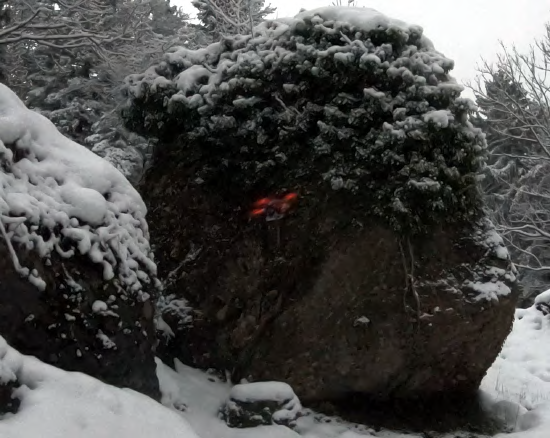
\includegraphics[keepaspectratio=true, width=\textwidth]{Navigation Environment/rocks.png}
		\caption{Rock}
	\end{subfigure}
	\hfill
	\begin{subfigure}[b]{0.29\textwidth}
		\centering
		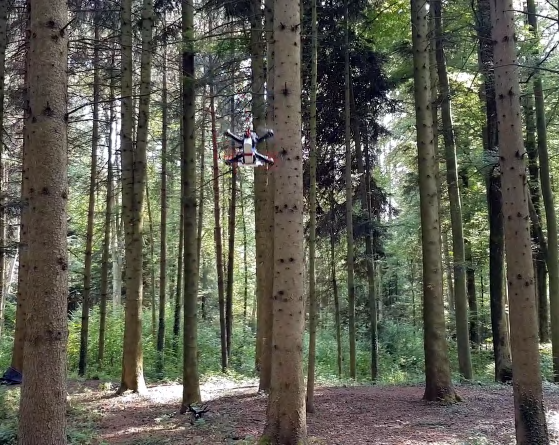
\includegraphics[keepaspectratio=true, width=\textwidth]{Navigation Environment/thin trees.png}
		\caption{Thin trees}
	\end{subfigure}
	\hfill
	\begin{subfigure}[b]{0.29\textwidth}
		\centering
		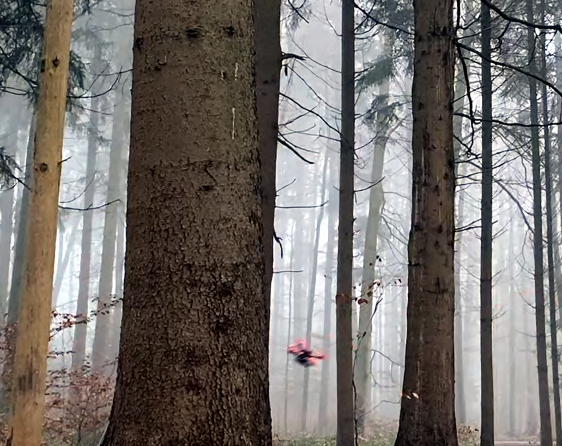
\includegraphics[keepaspectratio=true, width=\textwidth]{Navigation Environment/thik trees.png}
		\caption{Thick trees}
	\end{subfigure}
	\hfill
	\begin{subfigure}[b]{0.29\textwidth}
		\centering
		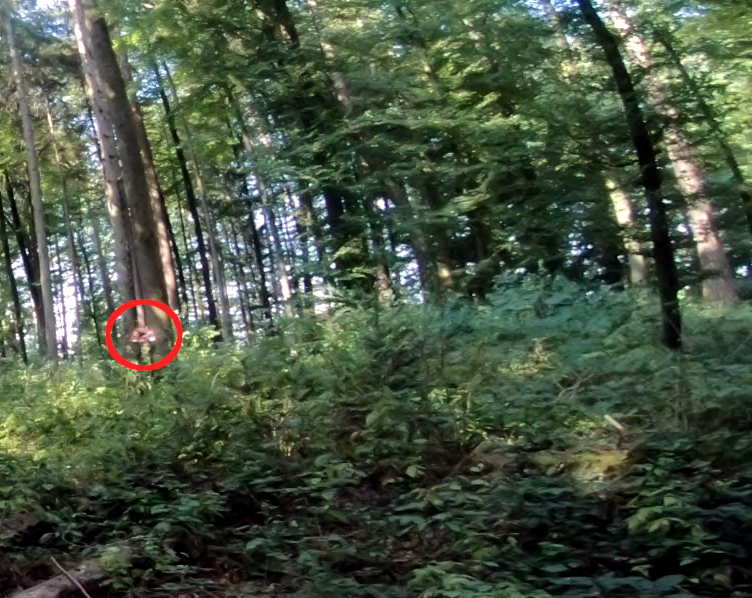
\includegraphics[keepaspectratio=true, width=\textwidth]{Navigation Environment/vegetation.png}
		\caption{Green vegetation}
	\end{subfigure}
	
	\caption{Natural environment test fields}
	\label{fig:natural envt}
\end{figure}

\textbf{Narrow gap test}\\
Here the drones are required to exit a hangar by passing through a narrow gap of about 0.8 m in width. At the start of the experiment, the drones are placed at about 10 m in front of and about 5 m to the right of the gap. The task was represented by a straight reference trajectory passing through a wall. This experiment is challenging since it requires a high-level understanding of the environment to turn early enough toward the gap. 

\subsection{Controlled experiments}
A set of controlled experiments in simulation was conducted to compare the performance of the model with several baselines. Two representative state-of-the-art approaches were selected as baselines for navigation in unknown environments: (i) FastPlanner \cite{fastPlanner} (ii) Reactive \cite{reactive_method}

The experiments was performed in the Flightmare simulator using the RotorS Gazebo plugin for accurate physics modeling and Unity as a rendering engine. The experiments are conducted in four different environments as shown in the figure \ref{fig:stimulated envt}. 

The drone is provided with the following: the state of the platform, depth measurements from the stereo camera \cite{stereoMatching}, and a goal in the form of a reference state that lies 5 s in the future. 

\begin{figure}[!h]
	\centering
	\begin{subfigure}[b]{0.48\textwidth}
		\centering
		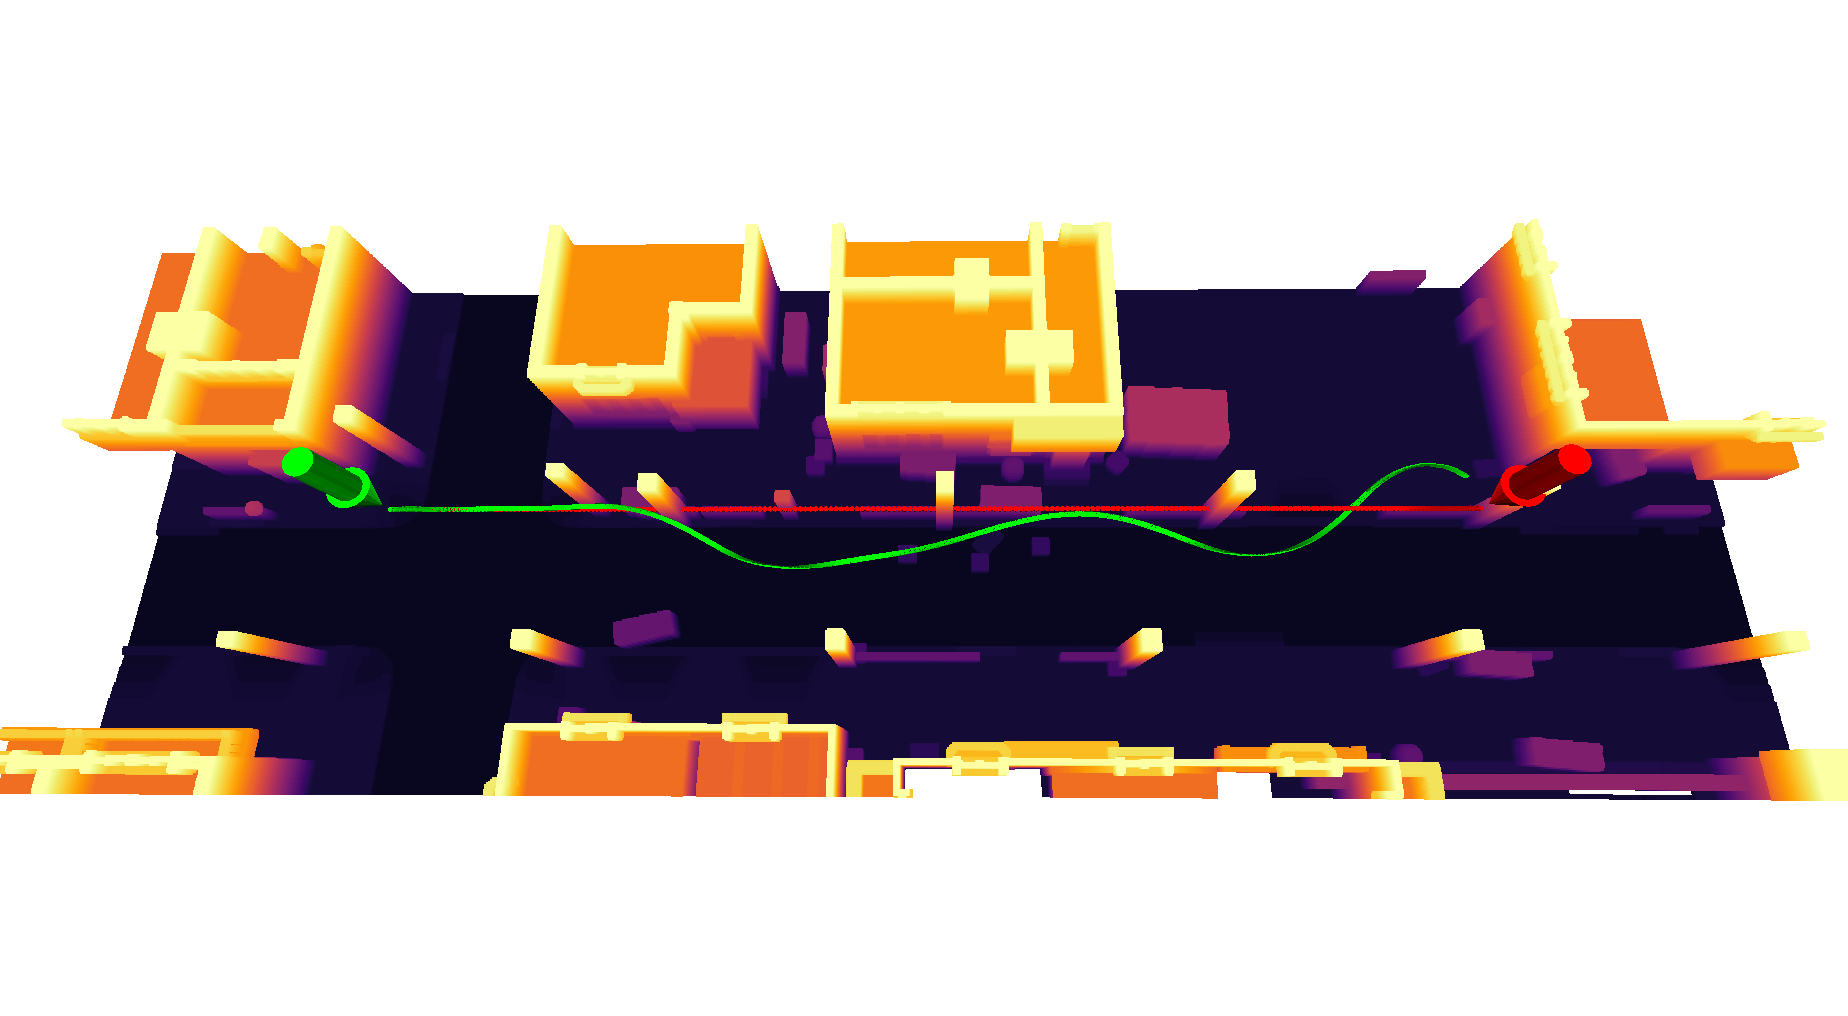
\includegraphics[keepaspectratio=true, width=\textwidth]{Navigation Environment/sti_city.png}
		\caption{Street City}
	\end{subfigure}
	\hfill
	\begin{subfigure}[b]{0.48\textwidth}
		\centering
		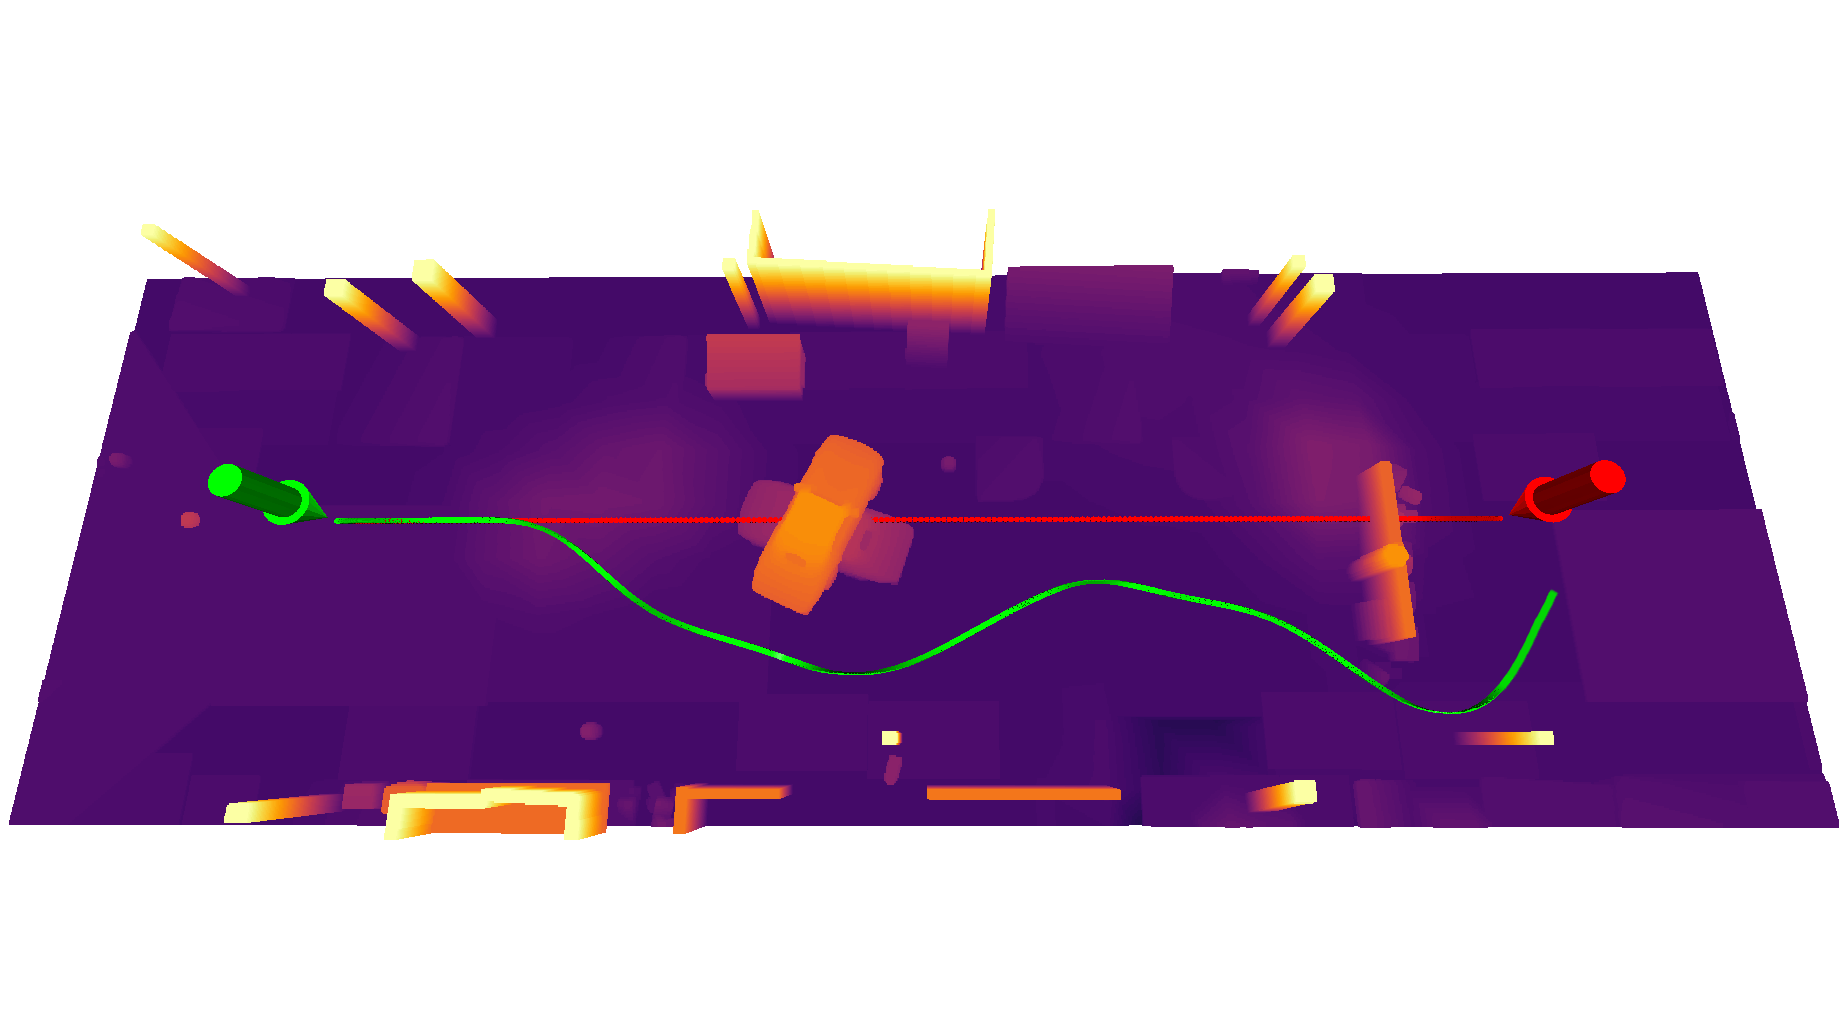
\includegraphics[keepaspectratio=true, width=\textwidth]{Navigation Environment/sti_disaster.png}
		\caption{Disasters (ruins)}
	\end{subfigure}
	\hfill	
	\begin{subfigure}[b]{0.48\textwidth}
		\centering
		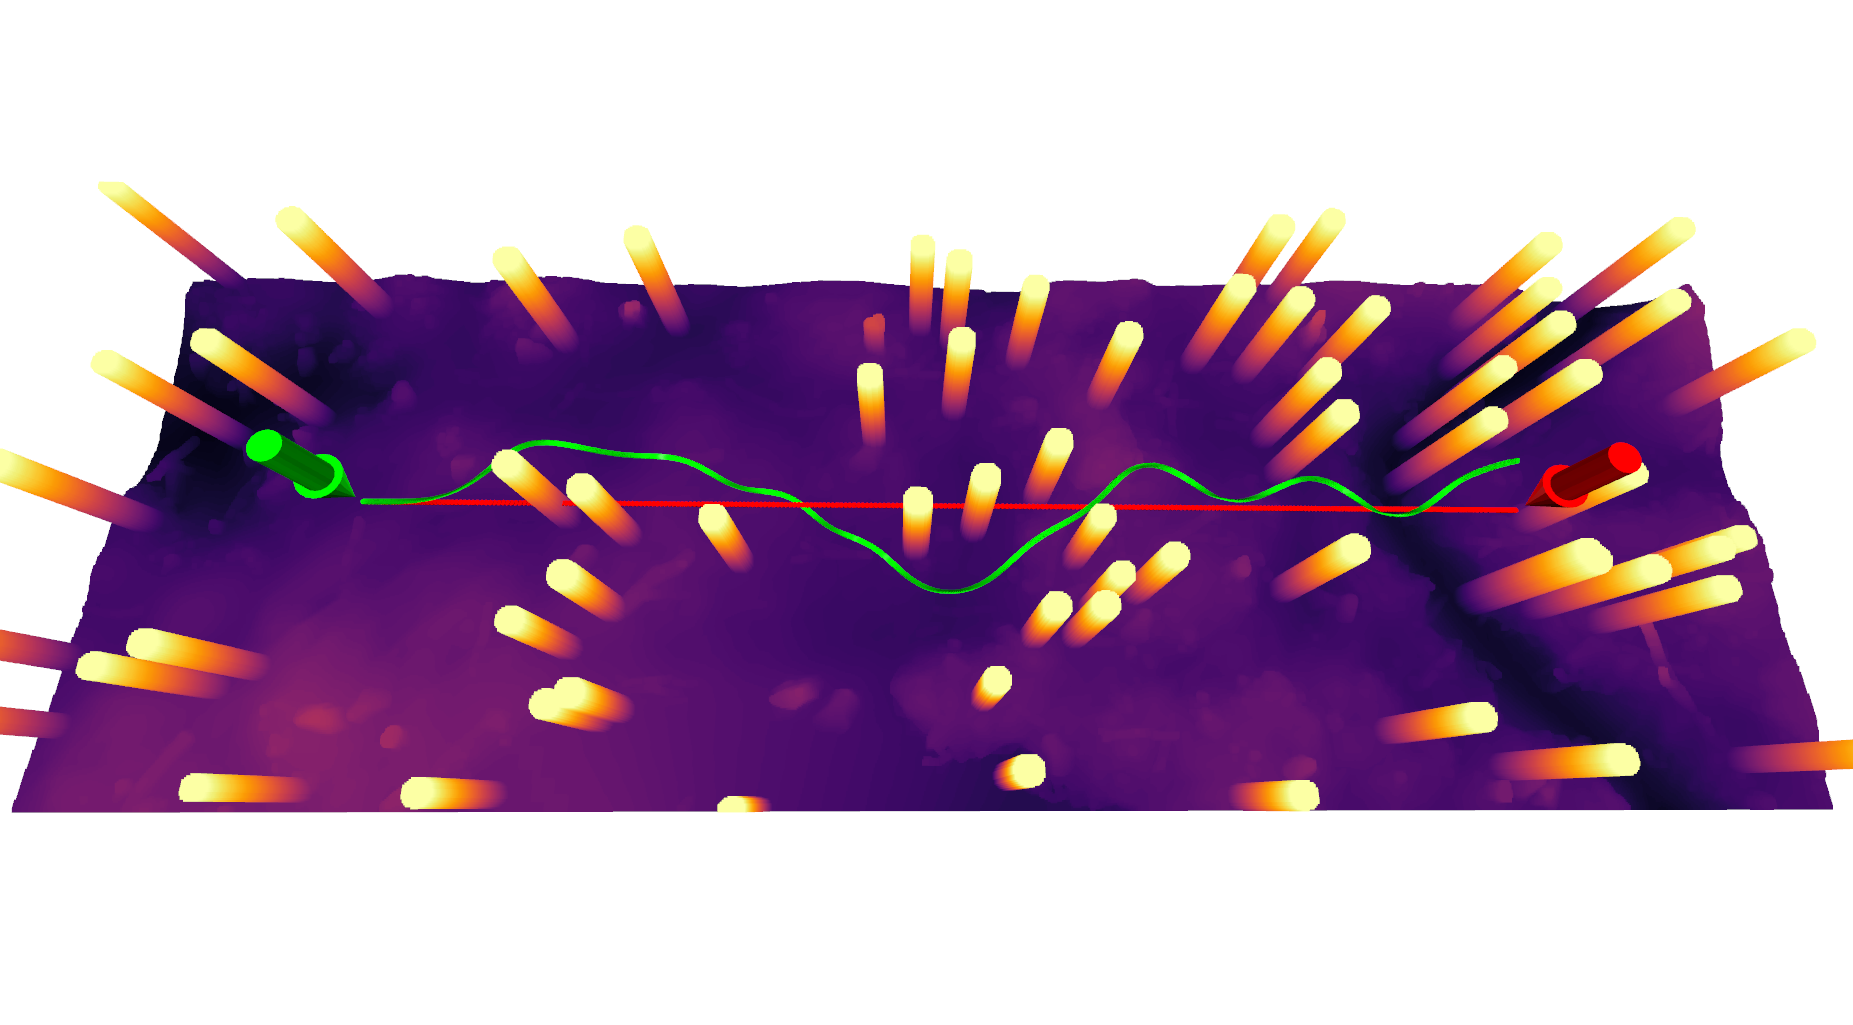
\includegraphics[keepaspectratio=true, width=\textwidth]{Navigation Environment/sti_forest.png}
		\caption{Forest}
	\end{subfigure}
	\hfill
	\begin{subfigure}[b]{0.48\textwidth}
		\centering
		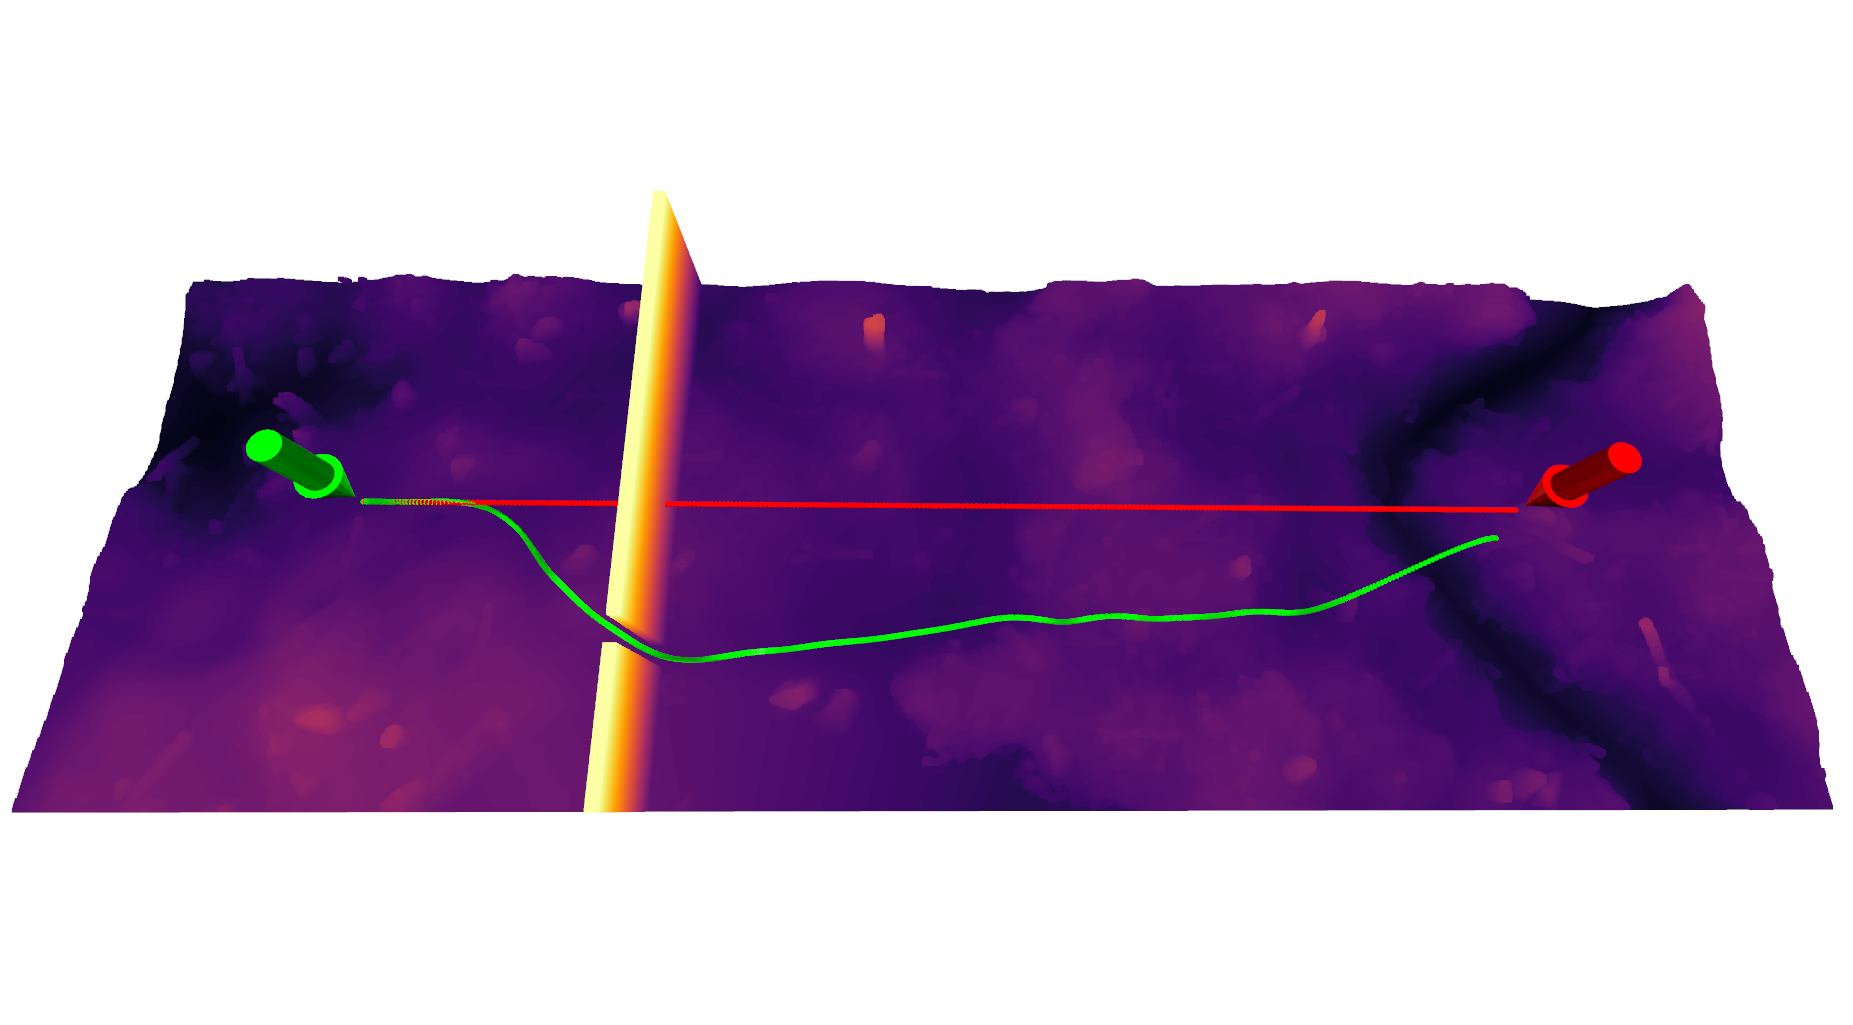
\includegraphics[keepaspectratio=true, width=\textwidth]{Navigation Environment/sti_narrow gap.png}
		\caption{Narrow gap}
	\end{subfigure}
	
	\caption{Stimulated environment test fields}
	\label{fig:stimulated envt}
\end{figure}


\section{Results}

\subsection{Natural environment}
Traditional mapping and planning approaches generally fail to achieve high speeds in such conditions, as both the thick vegetation and the texture-less snow terrain often cause very noisy depth observations. At average speeds of 3 and 5 $m/s$ the network consistently completed the task without experiencing a single crash. The state-of-the-art methods achieve in similar environments a maximum average speed of 2.29 $m/s$.

Despite the very high-speed of 5 to 7 $m/s$, the model successfully the maneuvered 8 out of 10 experiments. The two failures happened when objects entered the field of view very late because of the high angular velocity of the platform. At higher speed of 10 $m/s$, external disturbances, e.g. aerodynamics, battery power drops, and motion-blur start to play an important role and widen the simulation to reality gap. The results are summarized in the figure \ref{fig:natual-human-result}.

\subsection{Human-made environments}
A total of 19 experiments was performed with flight speeds in the range of 3 to 7 $m/s$. Given the lower success rate experienced in the forest environment at 10 $m/s$, test at higher speeds was not conducted to avoid fatal crashes. The results are summarized in the figure \ref{fig:natual-human-result}. 

\textbf{Narrow gap test}\\
The commercial drone, flying at a speed of about 2.7 $m/s$ consistently failed to pass through the gap across three experiments. On the other hand, the proposed model successfully flew through the narrow gap every time. A total of six experiments at flight speeds of 3 and 5 $m/s$ were conducted and the drone never experienced a crash.

\begin{figure}[!h]
	\begin{subfigure}[b]{0.38\textwidth}
		\centering
		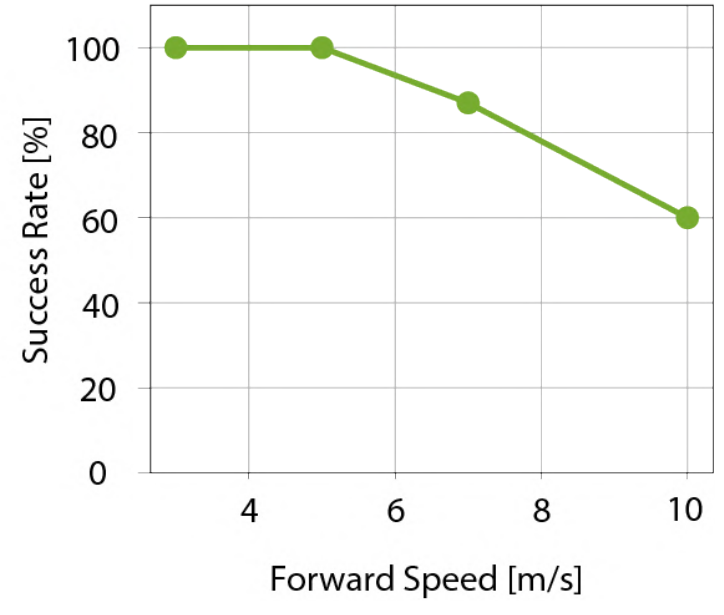
\includegraphics[keepaspectratio=true, width=\textwidth]{natural-human-linegraph.png}
		\caption{Cumulative results}
	\end{subfigure}
	\hfill
	\begin{subfigure}[b]{0.58\textwidth}
		\centering
		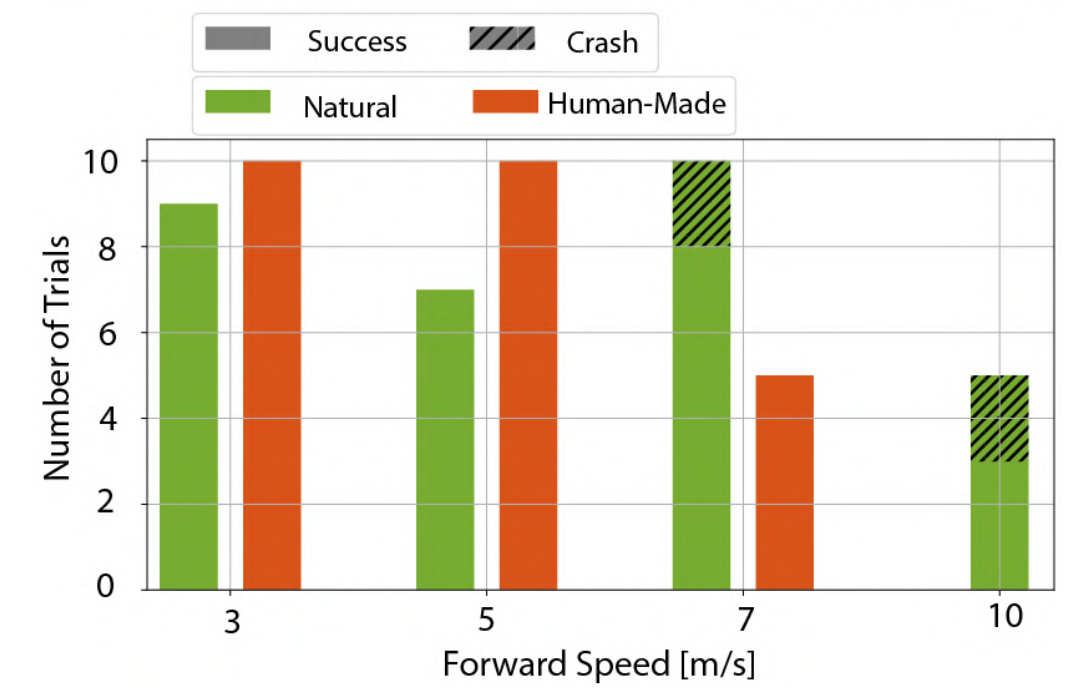
\includegraphics[keepaspectratio=true, width=\textwidth]{natural-human-bargraph.png}
		\caption{Trails}
	\end{subfigure}
	\caption{Natural and Human environment test results}
	\label{fig:natual-human-result}
\end{figure}

\subsection{Controlled experiments}
At low speeds (3 $m/s$ ) all methods perform similarly. However, as the speed increases, the baselines’ performances quickly drop: already at 5 $m/s$ , no baseline is able to complete all runs without crashing. In contrast, the proposed method can reliably fly at high-speeds through all environments, achieving an average success rate of 70 percent at 10 $m/s$ as shown in the figure \ref{fig:stimulated-results}. The drop in performance of the two baselines can be justified as follows.

\begin{itemize}
	\item Although the reactive \cite{reactive_method} baseline has a low processing latency, yet it has a limited expressive power: the trajectory to be executed can only be selected from a relatively small set of primitives. In addition, being the reactive \cite{reactive_method} baseline only conditioned on the current observation, it is strongly affected by noise in the observation.
	\item The FastPlanner \cite{fastPlanner} baseline can reject outliers in the depth map by leveraging multiple observations, which makes it more robust to sensing errors. However, this methods generally results in higher processing latency: Multiple observations are required to add obstacles in the map, and, therefore, to plan trajectories to avoid them. This problem is worsened by high-speed motion, which generally results in little overlap between consecutive observations.
\end{itemize}

\begin{figure}[!h]
	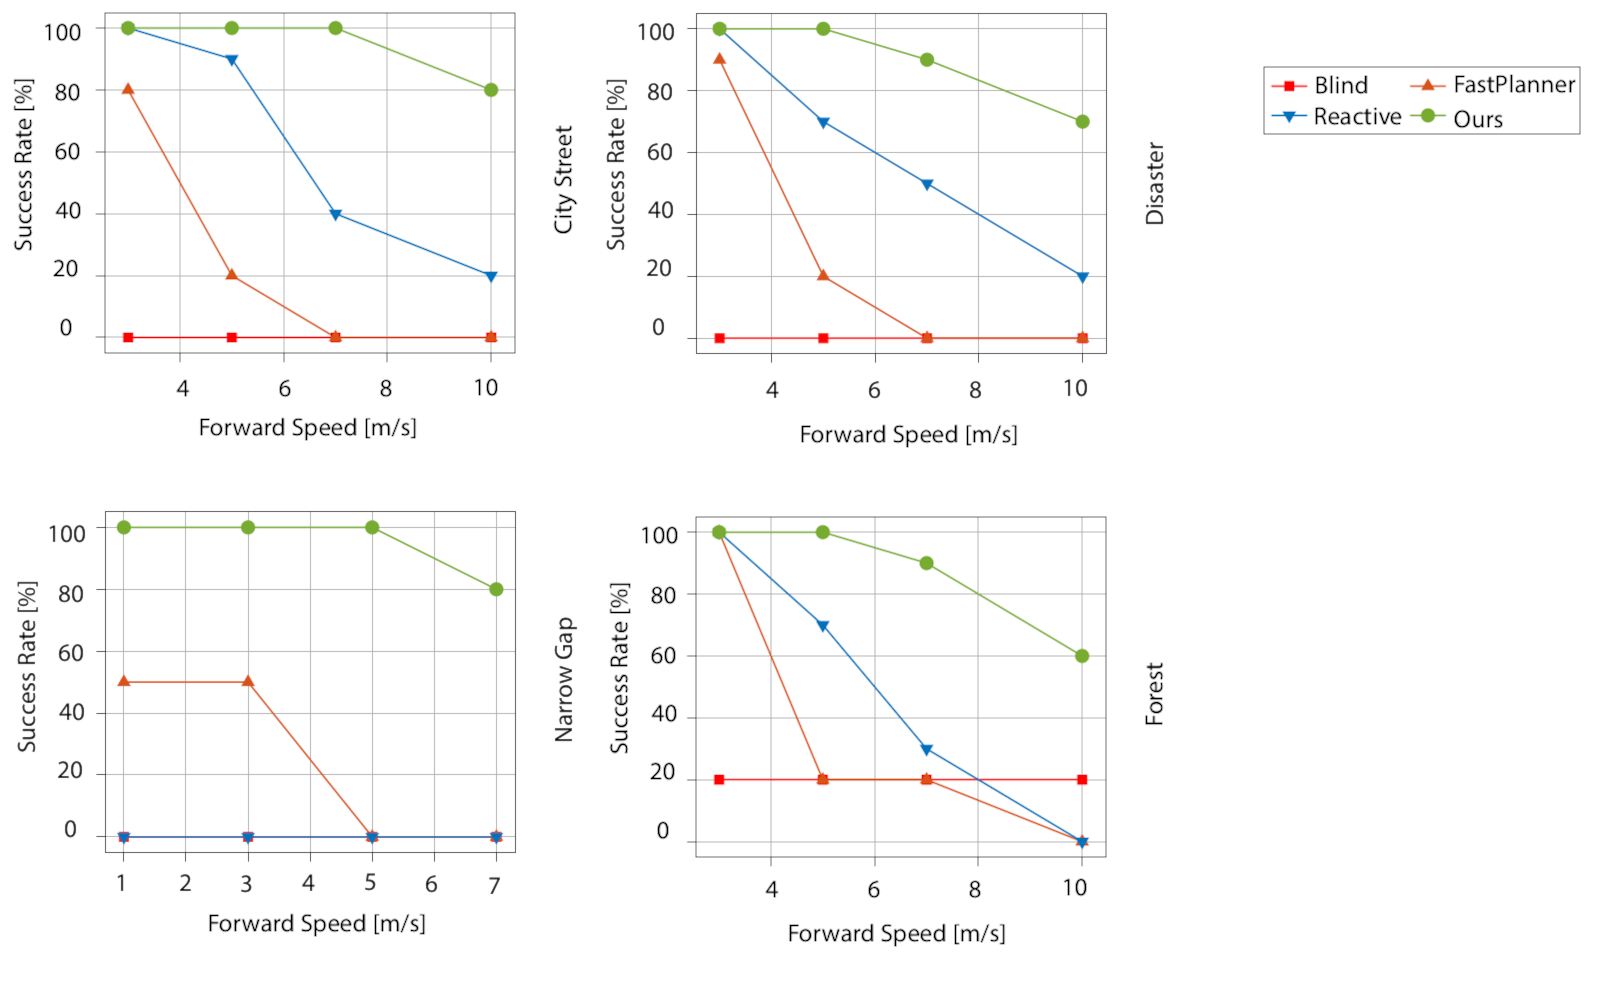
\includegraphics[width=\textwidth]{controlled-experiments.png}
	\caption{Controlled experiment results}
	\label{fig:stimulated_results}
\end{figure}


\section{Computational cost}
All timings were recorded on a desktop computer with a 6-core i7-8700 central processing unit (CPU), which was also used to run the simulation experiments. The timing are reported when using only the CPU for all approaches. The timings when performing neural network inference on a GeForce RTX 2080 graphics processing unit (GPU) is also recorded. Additionally, the timing of the algorithm on the onboard computer of the quadrotor (Jetson TX2) is also evaluated.

Table \ref{tab:processing-latency} shows the results of comparison of computational cost of the algorithm with the baselines. It highlights how each step of the methods contributes to the overall processing latency. 

\renewcommand{\arraystretch}{1.25}
\begin{table}[!h]
	\centering
	\resizebox{\textwidth}{!}{%
		\begin{tabular}{|c|c|cccc|}
			\hline
			Method &
			Components &
			$\mu$ (ms) &
			$\sigma$ (ms) &
			Perc. (\%) &
			\begin{tabular}[c]{@{}c@{}}Total Proc. \\ Latency (ms)\end{tabular} \\ \hline
			\multirow{3}{*}{FastPlanner \cite{fastPlanner}} & Pre-processing & 14.6        & 2.3        & 22.3 & \multirow{3}{*}{65.2} \\
			& Mapping        & 49.2        & 8.7        & 75.5 &                       \\
			& Planning       & 1.4         & 1.6        & 2.2  &                       \\ \hline
			\multirow{2}{*}{Reactive \cite{reactive_method}}    & Pre-processing & 14.6        & 2.3        & 22.3 & \multirow{2}{*}{19.1} \\
			& Planning       & 5.3         & 0.9        & 27.7 &                       \\ \hline
			\multirow{3}{*}{\begin{tabular}[c]{@{}c@{}}Proposed \\ model \cite{high-speed-flight}\end{tabular}} &
			Pre-processing &
			0.7 &
			0.04 &
			3.9 &
			\multirow{3}{*}{10.3 (2.6*)} \\
			& NN inference   & 10.1 (2.4*) & 1.5 (0.8*) & 93.0 &                       \\
			& Projection     & 0.08        & 0.01       & 3.1  &                       \\ \hline
			\multirow{3}{*}{\begin{tabular}[c]{@{}c@{}}Proposed\\ model \cite{high-speed-flight}\\ (Onboard)\end{tabular}} &
			Pre-processing &
			0.2 &
			0.01 &
			0.4 &
			\multirow{3}{*}{41.6} \\
			& NN inference   & 38.9        & 4.5        & 93.6 &                       \\
			& Projection     & 2.5         & 1.5        & 6.0  &                       \\ \hline
		\end{tabular}%
	}
	\caption[Processing Latency]{Processing Latency ($\mu$): The standard deviation $\sigma$ is computed over 1000 samples. The computation time is reported on the CPU and GPU (marked with *).}
	\label{tab:processing-latency}
\end{table}
\renewcommand{\arraystretch}{1}

With a total computation time of 65.2 ms per frame, FastPlanner \cite{fastPlanner} incurs the highest processing latency. The temporal filtering operations that are necessary to cope with sensing errors effectively make perception even slower. Two to three observations of an obstacle can be required to add it to the map, which increases the effective latency of the system. 

By foregoing the mapping stage altogether, the Reactive \cite{reactive_method} baseline significantly reduces computation time with a total processing latency of 19.1 ms. However, the reduced processing latency comes at the cost of the trajectory complexity that can be represented. In addition, the reactive\cite{reactive_method} baseline is sensitive to sensing errors, which can drastically affect performance at high speeds.
 

The proposed approach has significantly lower processing latency than both baselines; when network inference is performed on the GPU, the model is 25.3 times faster than FastPlanner \cite{fastPlanner} and 7.4 times faster than the Reactive baseline. When GPU inference is disabled, the network’s latency increases by only 8 ms. Moving from the desktop computer to the onboard embedded computing device, the network’s forward pass requires 38.9 ms. Onboard, the total time to pass from the sensor
reading to a plan is 41.6 ms, which corresponds to an update rate of about 24 Hz.


\section{Effect of latency and sensor noise}
In this experiment, the quadrotor travels along a straight line at a constant forward speed and is required to laterally evade a single obstacle (a pole) while having only limited sensing range. 

Upper-bound for the forward speed at which a robot can fly and avoid a single obstacle as a function of perception latency and sensing range is given by
\begin{equation}
	v_{max} = \frac{s}{t_s + t_p + t_{rot} + \sqrt{\frac{2*r_{obs}}{sin(\theta)*c_{max}}}}
\end{equation}

Where
\begin{itemize}
	\item $s$ : Sensing range
	\item $r_{obs}$ : The combined radius of the obstacle and the drone
	\item $t_s$ : The sensing latency,
	\item $t_p$ : The processing latency (the time to convert an observation into motor commands)
	\item $t_{rot}$ : The latency introduced to reorient the platform
	\item $\theta$ : The desired roll angle
	\item $c_{max}$ : The maximum mass-normalized thrust of the platform
\end{itemize}

The maximum speed depends on the sensing range, i.e. how far can an obstacle be accurately perceived, the latency of the visual sensor, i.e. the inverse of the frame rate, and the processing latency, i.e. the time to convert an observation into motor commands. 

The experiment is set up by placing a quadrotor with an initial forward velocity $v$ at a distance of $6 m$ from a pole with diameter $1.5 m$. The quadrotor is modeled as a sphere with radius $0.2 m$. The controlled experiment with varying forward speeds $v$ in the range of 3 to $13 m/s$ is then performed.

Ten experiments for each speed with all approaches are conducted and their success rates are reported. The experiment is executed in two settings: (i) with ground-truth depth information, to isolate the effect of latency on performance, and (ii) with depth estimated by stereo matching \cite{stereoMatching} (see fig \ref{fig:sterio-vision}) to analyze the effect of sensing errors to performance. The results are summarized in the figure \ref{fig:noise-graph}.

\subsection{Ground-truth depth}
All approaches can complete the task perfectly up to 5$m/s$ . However, even in these ideal conditions, the performance of the baselines drops for speeds beyond 5$m/s$ . This drop in performance for Reactive \cite{reactive_method} is because the finite library of motion primitives does not contain maneuvers that are aggressive enough to complete this task. Similarly, the performance degrades for FastPlanner \cite{fastPlanner} as a result of sub-optimal planning of actions. 

The proposed network can successfully avoid the obstacle without a single failure up to 7 $m/s$. For higher speeds, performance gracefully degrades to 60 percent at 10 $m/s$. This decrease in performance can be attributed to the sensitivity to imperfect network predictions when flying at high speed, where a single wrong action can lead to a crash. 

\subsection{Estimated depth}
The same experiment is repeated to study the influence of imperfect sensory measurements on performance. In this experiment, all methods are provided with depth maps that have been computed from the stereo pairs.   

The baselines experience a significant drop in performance compared with when provided with perfect sensory readings. FastPlanner \cite{fastPlanner} completely fails for speeds of 5 $m/s$ and beyond. This sharp drop in performance is because of the need for additional filtering of the noisy depth measurements.Similarly, the performance of the Reactive baseline drops by 30 percent at 7 $m/s$.

The network is only marginally affected by the noisy depth readings, with only a 10 percent drop in performance at 10 $m/s$, but no change in performance at lower speeds. This is because the sensorimotor policy, trained on depth from stereo, learns to account for common issues in the data such as discretization
artifacts and missing values. 

\begin{figure}[!h]
	\centering
	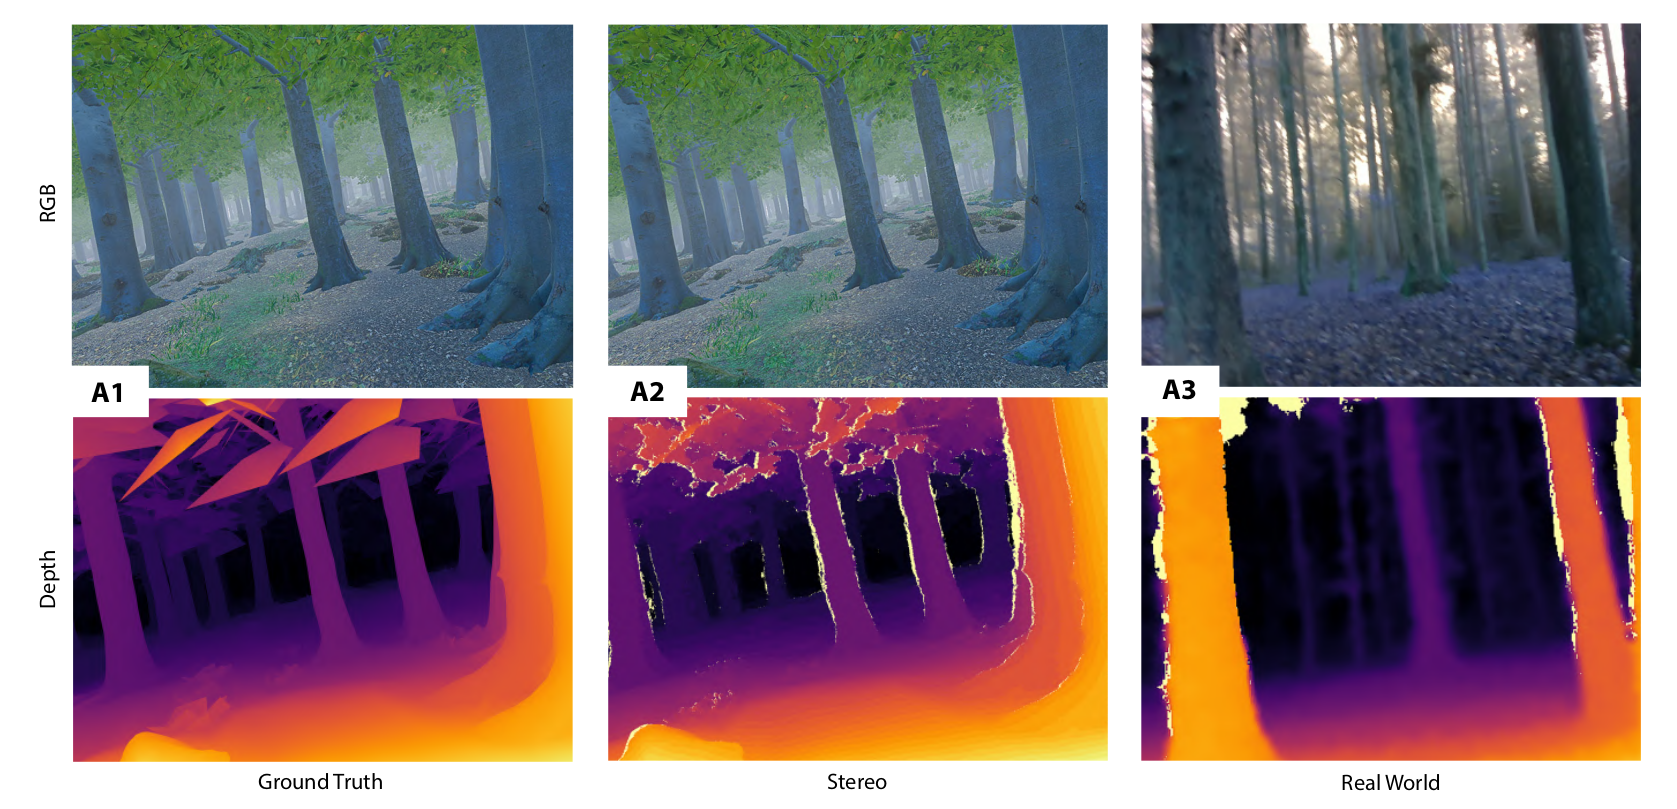
\includegraphics[width=\textwidth]{stimulation and stereo.png}
	\caption{Stereo vision into drone}
	\label{fig:sterio-vision}
\end{figure}

\begin{figure}[!h]
	\centering
	\begin{subfigure}[b]{0.75\textwidth}
		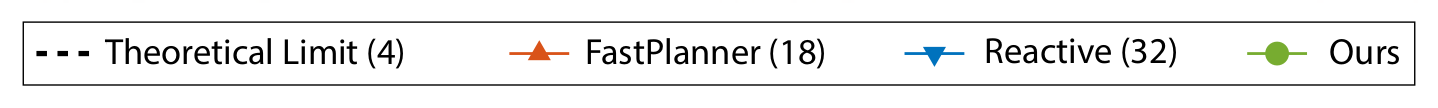
\includegraphics[width=\textwidth]{noise-graph(marker).png}
	\end{subfigure}
	\begin{subfigure}[b]{0.48\textwidth}
		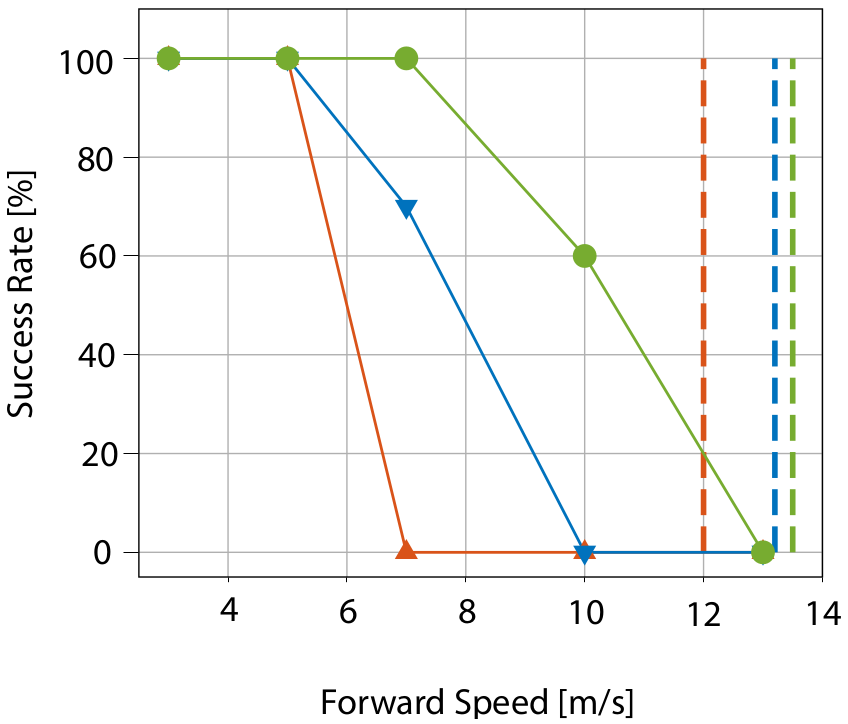
\includegraphics[width=\textwidth]{noise-graph(ground truth).png}
		\caption{Ground truth}
	\end{subfigure}
	\begin{subfigure}[b]{0.48\textwidth}
		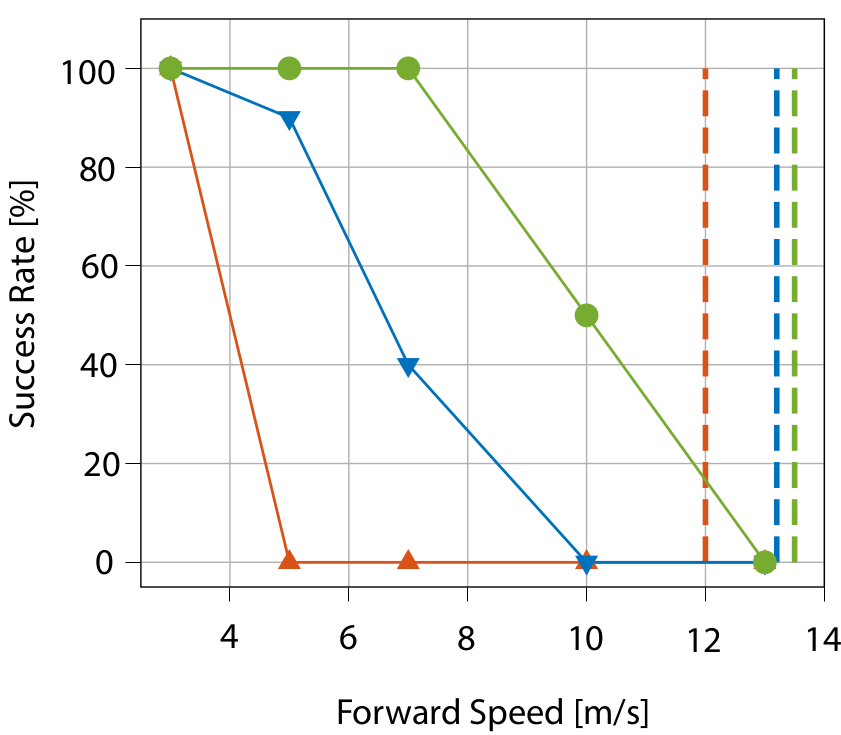
\includegraphics[width=\textwidth]{noise-graph(estimated depth).png}
		\caption{Estimated depth}
	\end{subfigure}
	\caption{Effect of Noise in performance}
	\label{fig:noise-graph}
\end{figure}